\section{Ejercicio 1}
\subsection{Problema: Tel\'egrafo}

La comunicacion es el progreso! decididos a entrar de lleno en la nueva era el pais decidio conectar telegraficamente todas las estaciones del moderno sistema ferreo que recorre el pais en abanico con origen en la capita (el kilometro 0). Por lo escaso del presupuesto, se ha decidido ofrecer cierta cantidad de kilometros de cable a cada ramal. Pero para maximizar el impacto en epocas electorales se busca lograr conectar la mayor cantidad de ciudades con los metros asignados (sin hacer cortes en el cable).\\

 Se busca optimizar las conexiones entre estaciones de un sistema de trenes. Para esto contamos con los siguientes datos:\\   
 
 El sistema est\'a dividido en ramales.
 
 Cada ramal comienza en la capital, que se encuentra en el kil\'ometro 0.
 
 En cada ramal contamos con una cantidad de cable para conectar estaciones.
 
 Se busca conectar la mayor cantidad de estaciones para cada ramal, sabiendo que el cable conector no puede dividirse.\\
 
 Se nos pide devolver por cada ramal un entero con la cantidad m\'axima de estaciones conectables respetando la complejidad $\bigO (n)$ siendo $n$ la cantidad de estaciones del sistema.

\subsubsection{Ejemplos}

\begin{table}[htb]
\centering
\begin{tabular}{|l|c|}
\hline
\multicolumn{1}{|c|}{Lineas Entrada}  & \multicolumn{1}{l|}{Linea Salida} \\ \hline
6                                     & \multirow{2}{*}{3}                \\ \cline{1-1}
6 8 12 15                             &                                   \\ \hline
35                                    & \multirow{2}{*}{6}                \\ \cline{1-1}
8 14 20 40 45 54 60 67 74 89 99       &                                   \\ \hline
100                                   & \multirow{2}{*}{4}                \\ \cline{1-1}
35 87 141 163 183 252 288 314 356 387 &                                   \\ \hline
90                                    & \multirow{2}{*}{14}               \\ \cline{1-1}
6 8 16 19 28 32 37 45 52 60 69 78 82  &                                   \\ \hline
4                                     & \multirow{2}{*}{0}                \\ \cline{1-1}
5 13 19 26 35                         &                                   \\ \hline
5                                     & \multirow{2}{*}{2}                \\ \cline{1-1}
5 13 19 26 35                         &                                   \\ \hline
5                                     & \multirow{2}{*}{2}                \\ \cline{1-1}
7 16 19 27 33                         &                                   \\ \hline
8                                     & \multirow{2}{*}{4}                \\ \cline{1-1}
2 5 8 14 18                           &                                   \\ \hline
8                                     & \multirow{2}{*}{3}                \\ \cline{1-1}
3 6 9 15 19                           &                                   \\ \hline
\end{tabular}
\caption{Ejemplos Tel\'egrafo}
\label{my-label}
\end{table}


\pagebreak
\subsection{Desarrollo}


 Para comenzar, tengamos en cuenta que el cable no puede dividirse, es decir que las estaciones conectadas deben ser consecutivas. Sabiendo esto, encaramos el problema mediante un algoritmo goloso.
 
 
 La idea es conectar todas las estaciones consecutivas posibles en un arreglo hasta que no tengamos mas cable disponible.\\
 
 Comenzamos recorriendo las estaciones pasadas por par\'ametro en orden, partiendo de una estaci\'on central imaginaria en el kilometro 0 y conectando cada una con su siguiente.
 
 Cuando decimos que $"conectamos"$ una estaci\'on con la siguiente, lo que hacemos en realidad es restarle al cable disponible la distancia entre ambas (su distancia es a la vez la resta entre el entero que representa a la estaci\'on siguiente menos el entero que representa a la estaci\'on actual).
 
 Si recorremos todas las estaciones con el cable disponible, devolveremos la cantidad total de estaciones mas uno (por la estaci\'on central); si esto no sucede es porque nos quedamos sin cable, es decir a la hora de conectar una estaci\'on con la siguiente, la distancia entre ambas fue mayor al cable restante.
 
 Cuando esto ocurra, tendremos que verificar que obtuvimos la mayor cantidad de estaciones conectables de la siguiente forma:
 
 Guardar la m\'axima cantidad de estaciones conectables obtenida hasta ahora y desconectar la primer estaci\'on del arreglo para asi intentar conectar la proxima estaci\'on (si es que existe) con el cable ahora sobrante despu\'es de desconectar la primera del arreglo.
 
 Si la distancia a la proxima estaci\'on (si es que existe) es mayor al cable restante, seguiremos desconectando de a una las estaciones del arreglo (siempre desconectando la primera) para obtener m\'as cable y reintentar conectar.\\
 Puede ocurrirr que la distancia a la pr\'oxima estaci\'on a conectar sea mayor que la cantidad de cable disponible (inclusive luego de desconectar todas las del arreglo). Si esto sucede, comenzaremos a completar el arreglo con el mismo metodo partiendo desde esta estaci\'on.\\
 
 Cuando lleguemos a la \'ultima estaci\'on, devolveremos el m\'aximo entre la cantidad de estaciones en el arreglo de estaciones conectadas actual y la m\'axima cantidad que fuimos guardando cada vez que nos qued\'abamos sin cable.
 
 
\pagebreak

\subsection{Justificaci\'on y Complejidad}

 Utilizaremos dos sub\'indices para recorrer las estaciones del problema. Ambos comienzan seteados en 0, o sea en la posici\'on de la estaci\'on central. Uno corresponde a la primera estaci\'on conectada en el arreglo actual de estaciones conectadas, $(A)$, y otro a la \'ultima estaci\'on conectada o agregada al arreglo de estaciones conectadas, $(B)$. 
 
El algoritmo termina cuando el \'indice $(B)$ llega a la \'ultima estaci\'on. Esto puede ocurrir de varias maneras y aunque el algoritmo tiene complejidad lineal, hay un mejor y peor caso:

\begin{enumerate}
    \item O bien la cantidad de cable inicial alcanz\'o para recorrer todas las estaciones y el algoritmo termina luego de hacer n conexiones.
    \subitem Este es el mejor caso ya que se recorren las n estaciones y se devuelve la mayor cantidad conectable en $\bigO(n)$.
    
    \item O se hacen uno o m\'as guardados de la m\'axima cantidad de estaciones conectadas actualmente y se comienza con un nuevo arreglo de estaciones conectadas.
    
    \subitem Este es el peor caso; ya que si bien el problema se resuelve en tiempo lineal $\bigO(n)$, se realizan hasta el doble de operaciones que en el caso anterior. 
\end{enumerate}
    
Veamos el peor caso posible: \\
    
     Imaginemos que tenemos n estaciones: n-1 estaciones en los kil\'ometros {1,2...n-1} y la \'ultima en el kil\'ometro  2n. Tambien supongamos que tenemos n kil\'ometros de cable. Nuestro algoritmo conectar\'ia las estaciones 1 a n-1 en n-1 pasos. Sin embargo, cuando intente conectar n-1 con n, tardar\'a n pasos en ver que es imposible; para luego comenzar otro arreglo en la \'ultima estaci\'on de la entrada de par\'ametros y terminar.\\


A continuaci\'on analizaremos el algoritmo:
\begin{description}
    Algoritmo 1.1 - Vista general - parametros: estaciones[], cableRestante
    \begin{verbatim}
    FOR i desde 1 hasta estaciones.length()  // O(n)
        distanciaActual = estaciones[i] - estaciones[i-1] //  O(1)
    
        IF cableRestante - distanciaActual >= 0
            .
            Algoritmo 1.2
            .
        ELSE
            .
            Algoritmo 1.3
            .
        ENDIF
    ENDFOR
    IF max > 0 : // O(1)
        max++  // O(1)
    ENDIF
    \end{verbatim}
\end{description}    
    
El bucle general recorre el arreglo linealmente, por lo que hasta el momento lleva $\bigO(n)$.
Veamos que ocurre en el algoritmo 1.2:

\begin{description}
    Algoritmo 1.2
    \begin{verbatim}
        cableRestante -= distanciaActual  // O(1)
        cantEstaciones++  // O(1)
        max = maximo(max, cantEstaciones) //  O(1)
        ultimaEstacionSumo[i-1] = true //  O(1)
        i++;  O(1)
    \end{verbatim}
\end{description}

En el caso de que con el cable que tenemos podamos agregar la proxima estaci\'on, simplemente se agrega y se resta al cable.
La complejidad de este caso es $\bigO(1)$ por lo que hasta el momento seguimos teniendo $\bigO(n)$

veamos el algoritmo 1.3:
\begin{description}
    Algoritmo 1.3
    \begin{verbatim}
         WHILE cableRestante - distanciaActual <= 0 && ultimaEstacion < i // O(n)
            IF ultimaEstacionSumo[ultimaEstacion] // O(1)
                distanciaASacar = estaciones[ultimaEstacion+1] -
                estaciones[ultimaEstacion]  // O(1)
                
                cableRestante += distanciaASacar // O(1)
                cantEstaciones-- // O(1)
            ENDIF
            ultimaEstacion++ // O(1)
        ENDWHILE
        IF ultimaEstacion == i // O(1)
            i++ //  O(1)
        ENDIF
    \end{verbatim}
\end{description}

a simple vista parece ser $\bigO(n)$ este caso, con lo que quedaria peor caso $\bigO(n^2)$ la soluci\'on, pero observando la condici\'on del bucle podemos ver que pide $ultimaEstacion < i$ por lo que no ira mas alla del indice en el que se encuentre el bucle exterior(algoritmo 1.1) y la variable $ultimaEstacion$ siempre avanza, por lo tanto este bucle hara como mucho $n$ pasos en el tiempo total en que corra el algoritmo. dado que es sobre el total de tiempo de corrida del algoritmo 1.1 lo tomaremos como una suma con respecto al bucle exterior, con esto la complejidad queda:\newline

\begin{center}
    $\bigO(n + n)$ \newline \newline
    $\bigO(2n)$ \newline \newline
    $\bigO(n)$ \newline \newline
\end{center}

Que es lo que queriamos demostrar.

\subsection{Correctitud}     
Probemos el algoritmo por inducci\'on \newline
Quiero probar P(n) = $(\forall n : entero > 0$) mi algoritmo devuelve la mayor cantidad de las n+1 estaciones consecutivas que se puedan conectar con una distancia de cable determinada o de no poder hacerlo devuelva cero. \newline
Veamos el caso base, n=1: \newline
resto estaciones[1] con estaciones[0] y pregunto si el cable alcanza.\newline

\begin{enumerate}
    \item De alcanzar (algoritmo 1.2) agrego esa estaci\'on y pasa a ser la mas larga hasta el momento, luego termina el agoritmo ya que no vuelve a cumplir la condici\'on del algoritmo 1.1. El resultado son dos estaciones. \newline
    \item De no alcanzar (algoritmo1.3) entro en el bucle, la primera condici\'on se cumple autom\'aticamente por hip\'otesis de este caso, y como entra con i = 1, \'ultima estaci\'on ser\'a 0, por lo que la condici\'on da true y pasa. Como el arreglo ultimaEstacion empieza en false, no se cumple la condici\'on y paso a sumar a ultimaEstacion, como esta es igual a i sumo 1 a i y vuelvo al bucle exterior. En este momento la condici\'on no se cumple y sale, dando como resultado cero estaciones. 
\end{enumerate}

Con esto queda probado que el caso base funciona, nuestra hip\'otesis inductiva sera que mi algoritmo funciona para $p(n)$, ahora suponiendo que vale $p(n)$ veamos si vale para $p(n+1)$.\newline \newline
Primero podemos observar que el arreglo contiene $n+2$ elementos, los cuales pueden ser tomados como un arreglo de $n+1$ elementos concatenado con el elemento $n+2-esimo$, sabiendo esto puedo aplicar mi hip\'otesis inductiva sobre el arreglo de $n+1$ elementos y comenzar la demostraci\'on en el elemento $n+2-esimo$ en el algoritmo 1.1, por hi\'potesis inductiva hasta el momento $\exists\ s : entero$ una posible soluci\'on maxima que conecta $k$ estaciones, con $0<= k <= n$ y hay una cantidad de cable dispnible $m$ con $0<= m <= cablemaximo$. sigamos con el algoritmo: \newline

El elemento entra al bucle del algoritmo 1.1, pasa ya que es el ultimo elemento, calculo la distancia entre la $n+1-esima$ y $n+2-esima$ estaciones, ahora:
\begin{enumerate}
    \item Si es menor a $m$, agrego esta estaci\'on, sumo uno mas y en la proxima iteracion salgo: \newline
    \begin{enumerate}
    \item si el maximo local que se estaba calculando hasta la anterior iteracion mas la nueva estaci\'on es mayor a $s$, entonces el maximo sera el maximo local mas uno, ya que agregue la nueva estaci\'on.
    \item si el maximo local que se estaba calculando hasta la anterior iteracion mas la nueva estaci\'on es menor o igual $s$, entonces el maximo sera $s$.
    \end{enumerate}
    
    \item si no, entro en el else y comienzo a sacar estaciones del princio de la subsolucion actual:
    \begin{enumerate}
    \item Si saco todas las estaciones que tenia hasta el momento, me quedara solo la nueva estaci\'on que agregue, con lo que significa que no me alcanza el cable, suma uno a i y en la proxima iteracion del algoritmo 1.1 no entrara en el bucle principal, devolviendo el resultado $s$ previamente calculado.
    \item Si saco algunas de las estaciones que tenia hasta el momento, me quedara un subarreglo de estaciones y al salir del bucle, volvera a entrar en el algoritmo 1.1 entrando por la primer condici\'on y caera en el caso 1 de esta demostracion.
    \end{enumerate}
\end{enumerate}
Con esto vale $P(n+1)$. Luego $(\forall\ n : entero > 0$) mi algoritmo devuelve la mayor cantidad de las n+1 estaciones consecutivas que se puedan conectar con una distancia de cable determinada o de no poder hacerlo devuelve cero.\newline
Con esto queda demostrado que el algoritmo es correcto.

\subsection{Tests}
Para los Tests analizamos su mejor y peor caso.
    \subsubsection{Mejor Caso}
        El mejor caso es que nunca tenga que sacar estaciones de la subsolucion que este calculando, para esto armamos un arreglo cuya suma de distancias sea menor a la longitud maxima de cable, de esta manera siempre agrega siendo costo $\bigO(n)$. \newline
    \lstinputlisting[language=Java]{modulos/Tests_Code/testej1mejor.txt}
    
    \subsubsection{Peor Caso}
        El peor caso es cuando debe sacar todas las estaciones del arreglo ya que termina siendo costo $2 * \bigO(n)$, para esto armamos arreglos en donde la distancia entre todas las estaciones sea menor que la longitud total de cable excepto la ultima, cuya logitud es mayor que todo el cable, de esta manera, el algoritmo tendra que realizar 2*n operaciones. \newline
    \lstinputlisting[language=Java]{modulos/Tests_Code/testej1mejor.txt}
    
    \pagebreak
    
    \subsubsection{Performance}
    
    Observamos el contraste de nuestro peor y mejor caso. La variaci\'on en el peor caso est\'a en la constante 2 que multiplica a la cantidad de operaciones realiza en el mejor caso.
    
    \begin{figure}[h!]
    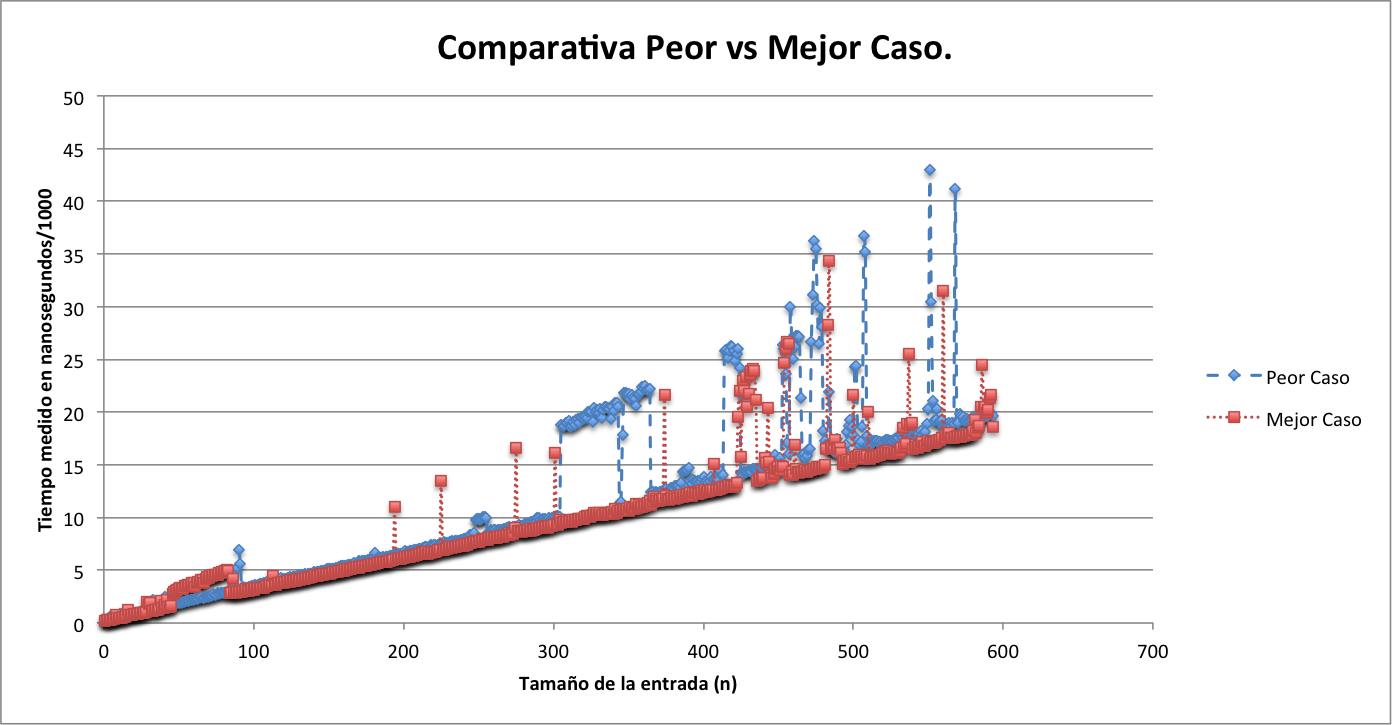
\includegraphics[width=140mm]{ejercicio1_mejorvspeor.png}
    \centering
    \caption{Comparativa Mejor vs Peor Caso}
    \label{overflow3}
    \end{figure}
    
        Se observa que nuestro mejor caso tiene un comportamiento lineal y mantiene ese comportamiento a medida que las entradas se hacen m\'as numerosas. 
    
    \begin{figure}[h!]
    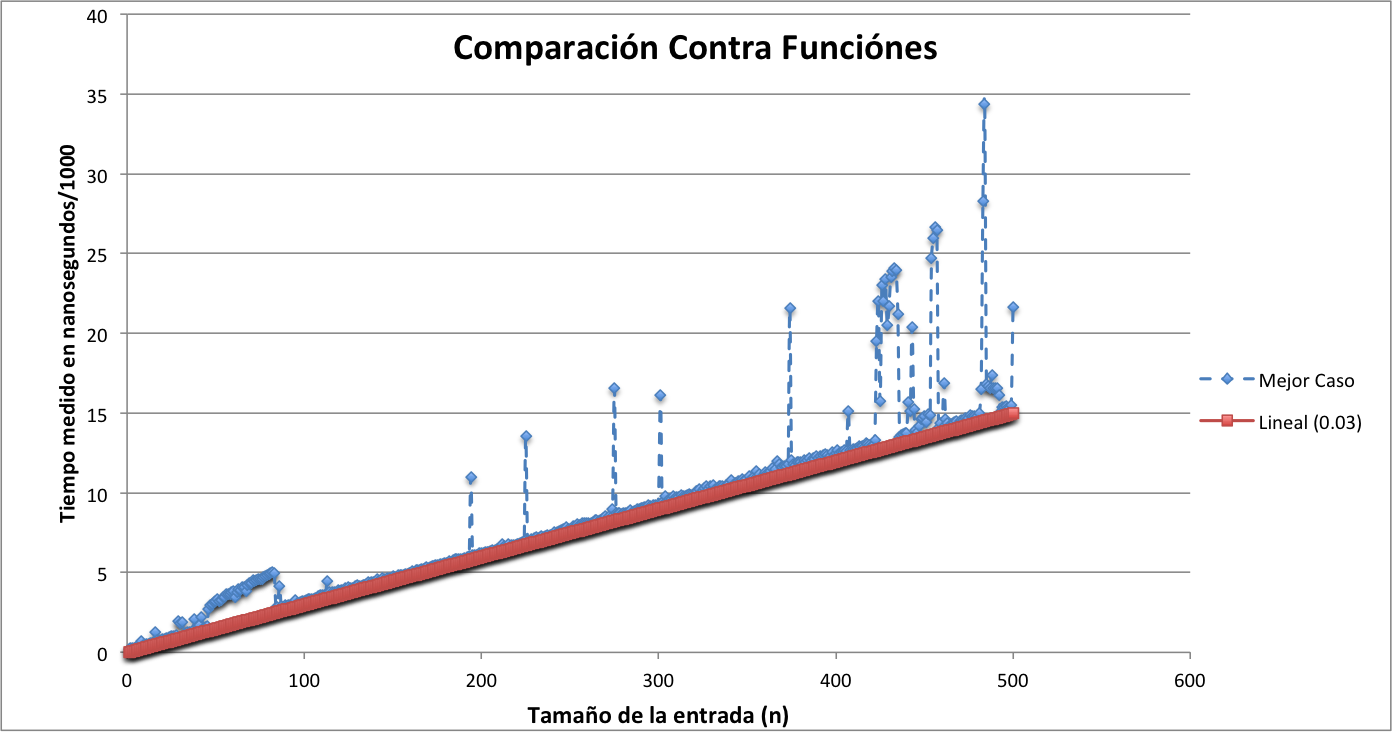
\includegraphics[width=140mm]{ejercicio1_comparativo.png}
    \centering
    \caption{Comparativa Contra Funcion Lineal, Cuadratica y constante}
    \label{overflow3}
    \end{figure}

\pagebreak